\documentclass[twoside]{book}

% Packages required by doxygen
\usepackage{calc}
\usepackage{doxygen}
\usepackage{graphicx}
\usepackage[utf8]{inputenc}
\usepackage{makeidx}
\usepackage{multicol}
\usepackage{multirow}
\usepackage{textcomp}
\usepackage[table]{xcolor}

% Font selection
\usepackage[T1]{fontenc}
\usepackage{mathptmx}
\usepackage[scaled=.90]{helvet}
\usepackage{courier}
\usepackage{amssymb}
\usepackage{sectsty}
\renewcommand{\familydefault}{\sfdefault}
\allsectionsfont{%
  \fontseries{bc}\selectfont%
  \color{darkgray}%
}
\renewcommand{\DoxyLabelFont}{%
  \fontseries{bc}\selectfont%
  \color{darkgray}%
}

% Page & text layout
\usepackage{geometry}
\geometry{%
  a4paper,%
  top=2.5cm,%
  bottom=2.5cm,%
  left=2.5cm,%
  right=2.5cm%
}
\tolerance=750
\hfuzz=15pt
\hbadness=750
\setlength{\emergencystretch}{15pt}
\setlength{\parindent}{0cm}
\setlength{\parskip}{0.2cm}
\makeatletter
\renewcommand{\paragraph}{%
  \@startsection{paragraph}{4}{0ex}{-1.0ex}{1.0ex}{%
    \normalfont\normalsize\bfseries\SS@parafont%
  }%
}
\renewcommand{\subparagraph}{%
  \@startsection{subparagraph}{5}{0ex}{-1.0ex}{1.0ex}{%
    \normalfont\normalsize\bfseries\SS@subparafont%
  }%
}
\makeatother

% Headers & footers
\usepackage{fancyhdr}
\pagestyle{fancyplain}
\fancyhead[LE]{\fancyplain{}{\bfseries\thepage}}
\fancyhead[CE]{\fancyplain{}{}}
\fancyhead[RE]{\fancyplain{}{\bfseries\leftmark}}
\fancyhead[LO]{\fancyplain{}{\bfseries\rightmark}}
\fancyhead[CO]{\fancyplain{}{}}
\fancyhead[RO]{\fancyplain{}{\bfseries\thepage}}
\fancyfoot[LE]{\fancyplain{}{}}
\fancyfoot[CE]{\fancyplain{}{}}
\fancyfoot[RE]{\fancyplain{}{\bfseries\scriptsize Generated on Sun May 10 2015 15\-:26\-:22 for My Project by Doxygen }}
\fancyfoot[LO]{\fancyplain{}{\bfseries\scriptsize Generated on Sun May 10 2015 15\-:26\-:22 for My Project by Doxygen }}
\fancyfoot[CO]{\fancyplain{}{}}
\fancyfoot[RO]{\fancyplain{}{}}
\renewcommand{\footrulewidth}{0.4pt}
\renewcommand{\chaptermark}[1]{%
  \markboth{#1}{}%
}
\renewcommand{\sectionmark}[1]{%
  \markright{\thesection\ #1}%
}

% Indices & bibliography
\usepackage{natbib}
\usepackage[titles]{tocloft}
\setcounter{tocdepth}{3}
\setcounter{secnumdepth}{5}
\makeindex

% Hyperlinks (required, but should be loaded last)
\usepackage{ifpdf}
\ifpdf
  \usepackage[pdftex,pagebackref=true]{hyperref}
\else
  \usepackage[ps2pdf,pagebackref=true]{hyperref}
\fi
\hypersetup{%
  colorlinks=true,%
  linkcolor=blue,%
  citecolor=blue,%
  unicode%
}

% Custom commands
\newcommand{\clearemptydoublepage}{%
  \newpage{\pagestyle{empty}\cleardoublepage}%
}


%===== C O N T E N T S =====

\begin{document}

% Titlepage & ToC
\hypersetup{pageanchor=false}
\pagenumbering{roman}
\begin{titlepage}
\vspace*{7cm}
\begin{center}%
{\Large My Project }\\
\vspace*{1cm}
{\large Generated by Doxygen 1.8.6}\\
\vspace*{0.5cm}
{\small Sun May 10 2015 15:26:22}\\
\end{center}
\end{titlepage}
\clearemptydoublepage
\tableofcontents
\clearemptydoublepage
\pagenumbering{arabic}
\hypersetup{pageanchor=true}

%--- Begin generated contents ---
\chapter{Namespace Index}
\section{Namespace List}
Here is a list of all documented namespaces with brief descriptions\-:\begin{DoxyCompactList}
\item\contentsline{section}{\hyperlink{namespaceratings_1_1forms}{ratings.\-forms} }{\pageref{namespaceratings_1_1forms}}{}
\item\contentsline{section}{\hyperlink{namespaceratings_1_1models}{ratings.\-models} }{\pageref{namespaceratings_1_1models}}{}
\item\contentsline{section}{\hyperlink{namespaceratings_1_1urls}{ratings.\-urls} }{\pageref{namespaceratings_1_1urls}}{}
\item\contentsline{section}{\hyperlink{namespaceratings_1_1views}{ratings.\-views} }{\pageref{namespaceratings_1_1views}}{}
\end{DoxyCompactList}

\chapter{Hierarchical Index}
\section{Class Hierarchy}
This inheritance list is sorted roughly, but not completely, alphabetically\-:\begin{DoxyCompactList}
\item \contentsline{section}{ratings.\-forms.\-Category\-Nomination\-Form.\-Meta}{\pageref{classratings_1_1forms_1_1CategoryNominationForm_1_1Meta}}{}
\item \contentsline{section}{ratings.\-forms.\-Vote\-Form.\-Meta}{\pageref{classratings_1_1forms_1_1VoteForm_1_1Meta}}{}
\item \contentsline{section}{ratings.\-forms.\-Tool\-Nomination\-Form.\-Meta}{\pageref{classratings_1_1forms_1_1ToolNominationForm_1_1Meta}}{}
\item Model\begin{DoxyCompactList}
\item \contentsline{section}{ratings.\-models.\-Category}{\pageref{classratings_1_1models_1_1Category}}{}
\item \contentsline{section}{ratings.\-models.\-Tool}{\pageref{classratings_1_1models_1_1Tool}}{}
\item \contentsline{section}{ratings.\-models.\-Tool\-Cat}{\pageref{classratings_1_1models_1_1ToolCat}}{}
\item \contentsline{section}{ratings.\-models.\-Vote}{\pageref{classratings_1_1models_1_1Vote}}{}
\end{DoxyCompactList}
\item Model\-Form\begin{DoxyCompactList}
\item \contentsline{section}{ratings.\-forms.\-Category\-Nomination\-Form}{\pageref{classratings_1_1forms_1_1CategoryNominationForm}}{}
\item \contentsline{section}{ratings.\-forms.\-Tool\-Nomination\-Form}{\pageref{classratings_1_1forms_1_1ToolNominationForm}}{}
\item \contentsline{section}{ratings.\-forms.\-Vote\-Form}{\pageref{classratings_1_1forms_1_1VoteForm}}{}
\end{DoxyCompactList}
\item renderer\begin{DoxyCompactList}
\item \contentsline{section}{ratings.\-forms.\-Horiz\-Radio\-Renderer}{\pageref{classratings_1_1forms_1_1HorizRadioRenderer}}{}
\end{DoxyCompactList}
\end{DoxyCompactList}

\chapter{Class Index}
\section{Class List}
Here are the classes, structs, unions and interfaces with brief descriptions\-:\begin{DoxyCompactList}
\item\contentsline{section}{\hyperlink{classratings_1_1models_1_1Category}{ratings.\-models.\-Category} }{\pageref{classratings_1_1models_1_1Category}}{}
\item\contentsline{section}{\hyperlink{classratings_1_1forms_1_1CategoryNominationForm}{ratings.\-forms.\-Category\-Nomination\-Form} }{\pageref{classratings_1_1forms_1_1CategoryNominationForm}}{}
\item\contentsline{section}{\hyperlink{classratings_1_1forms_1_1HorizRadioRenderer}{ratings.\-forms.\-Horiz\-Radio\-Renderer} }{\pageref{classratings_1_1forms_1_1HorizRadioRenderer}}{}
\item\contentsline{section}{\hyperlink{classratings_1_1forms_1_1CategoryNominationForm_1_1Meta}{ratings.\-forms.\-Category\-Nomination\-Form.\-Meta} }{\pageref{classratings_1_1forms_1_1CategoryNominationForm_1_1Meta}}{}
\item\contentsline{section}{\hyperlink{classratings_1_1forms_1_1VoteForm_1_1Meta}{ratings.\-forms.\-Vote\-Form.\-Meta} }{\pageref{classratings_1_1forms_1_1VoteForm_1_1Meta}}{}
\item\contentsline{section}{\hyperlink{classratings_1_1forms_1_1ToolNominationForm_1_1Meta}{ratings.\-forms.\-Tool\-Nomination\-Form.\-Meta} }{\pageref{classratings_1_1forms_1_1ToolNominationForm_1_1Meta}}{}
\item\contentsline{section}{\hyperlink{classratings_1_1models_1_1Tool}{ratings.\-models.\-Tool} }{\pageref{classratings_1_1models_1_1Tool}}{}
\item\contentsline{section}{\hyperlink{classratings_1_1models_1_1ToolCat}{ratings.\-models.\-Tool\-Cat} }{\pageref{classratings_1_1models_1_1ToolCat}}{}
\item\contentsline{section}{\hyperlink{classratings_1_1forms_1_1ToolNominationForm}{ratings.\-forms.\-Tool\-Nomination\-Form} }{\pageref{classratings_1_1forms_1_1ToolNominationForm}}{}
\item\contentsline{section}{\hyperlink{classratings_1_1models_1_1Vote}{ratings.\-models.\-Vote} }{\pageref{classratings_1_1models_1_1Vote}}{}
\item\contentsline{section}{\hyperlink{classratings_1_1forms_1_1VoteForm}{ratings.\-forms.\-Vote\-Form} }{\pageref{classratings_1_1forms_1_1VoteForm}}{}
\end{DoxyCompactList}

\chapter{Namespace Documentation}
\hypertarget{namespaceratings_1_1forms}{\section{ratings.\-forms Namespace Reference}
\label{namespaceratings_1_1forms}\index{ratings.\-forms@{ratings.\-forms}}
}
\subsection*{Classes}
\begin{DoxyCompactItemize}
\item 
class \hyperlink{classratings_1_1forms_1_1HorizRadioRenderer}{Horiz\-Radio\-Renderer}
\item 
class \hyperlink{classratings_1_1forms_1_1VoteForm}{Vote\-Form}
\item 
class \hyperlink{classratings_1_1forms_1_1CategoryNominationForm}{Category\-Nomination\-Form}
\item 
class \hyperlink{classratings_1_1forms_1_1ToolNominationForm}{Tool\-Nomination\-Form}
\end{DoxyCompactItemize}


\subsection{Detailed Description}
\begin{DoxyVerb}import django modules
\end{DoxyVerb}
 
\hypertarget{namespaceratings_1_1models}{\section{ratings.\-models Namespace Reference}
\label{namespaceratings_1_1models}\index{ratings.\-models@{ratings.\-models}}
}
\subsection*{Classes}
\begin{DoxyCompactItemize}
\item 
class \hyperlink{classratings_1_1models_1_1Tool}{Tool}
\item 
class \hyperlink{classratings_1_1models_1_1Category}{Category}
\item 
class \hyperlink{classratings_1_1models_1_1ToolCat}{Tool\-Cat}
\item 
class \hyperlink{classratings_1_1models_1_1Vote}{Vote}
\end{DoxyCompactItemize}


\subsection{Detailed Description}
\begin{DoxyVerb}Import django modules.
\end{DoxyVerb}
 
\hypertarget{namespaceratings_1_1urls}{\section{ratings.\-urls Namespace Reference}
\label{namespaceratings_1_1urls}\index{ratings.\-urls@{ratings.\-urls}}
}
\subsection*{Variables}
\begin{DoxyCompactItemize}
\item 
tuple {\bfseries urlpatterns}
\end{DoxyCompactItemize}


\subsection{Detailed Description}
\begin{DoxyVerb}import django modules
\end{DoxyVerb}
 

\subsection{Variable Documentation}
\hypertarget{namespaceratings_1_1urls_a2e8a8fea61824e88a8a18b13c0e3ce96}{\index{ratings\-::urls@{ratings\-::urls}!urlpatterns@{urlpatterns}}
\index{urlpatterns@{urlpatterns}!ratings::urls@{ratings\-::urls}}
\subsubsection[{urlpatterns}]{\setlength{\rightskip}{0pt plus 5cm}tuple ratings.\-urls.\-urlpatterns}}\label{namespaceratings_1_1urls_a2e8a8fea61824e88a8a18b13c0e3ce96}
{\bfseries Initial value\-:}
\begin{DoxyCode}
1 = patterns(\textcolor{stringliteral}{''},
2     \textcolor{stringliteral}{"""    define regex matches for URLs    """}
3     url(\textcolor{stringliteral}{r'^$'}, views.home),
4     url(\textcolor{stringliteral}{r'^categories$'}, views.categorys\_list),
5     url(\textcolor{stringliteral}{r'^nominate\_category$'}, views.nominate\_category),
6     url(\textcolor{stringliteral}{r'^nominate\_tool$'}, views.nominate\_tool),
7     url(\textcolor{stringliteral}{r'^category/(?P<pk>[0-9]+)/$'}, views.category\_detail),
8     url(\textcolor{stringliteral}{r'^category/(.+)/$'}, views.category\_detail\_by\_name),
9     url(\textcolor{stringliteral}{r'^tool/(.+)/$'}, views.tool\_detail\_by\_name),
10     url(\textcolor{stringliteral}{r'^tool/(?P<pk>[0-9]+)/$'}, views.tool\_detail),
11 )
\end{DoxyCode}

\hypertarget{namespaceratings_1_1views}{\section{ratings.\-views Namespace Reference}
\label{namespaceratings_1_1views}\index{ratings.\-views@{ratings.\-views}}
}
\subsection*{Functions}
\begin{DoxyCompactItemize}
\item 
def \hyperlink{namespaceratings_1_1views_a401b3d84faec578bfa116c19fa24ce67}{home}
\item 
def \hyperlink{namespaceratings_1_1views_ad512086421b30c0d5e1800034201b271}{nominate\-\_\-tool}
\item 
def \hyperlink{namespaceratings_1_1views_a7a946d0d957506dd5d6e1549d640139d}{categorys\-\_\-list}
\item 
def \hyperlink{namespaceratings_1_1views_abbd64ae210bb4d2379f8beda67368937}{category\-\_\-detail}
\item 
def \hyperlink{namespaceratings_1_1views_a9b9e82f2153c0cd0289192205cc788c6}{category\-\_\-detail\-\_\-by\-\_\-name}
\item 
def \hyperlink{namespaceratings_1_1views_a6218c4e7c538409fc2db4f4a3f67864c}{tool\-\_\-detail\-\_\-by\-\_\-name}
\item 
def \hyperlink{namespaceratings_1_1views_a8638da26f9b08f21106113d3139c8938}{tool\-\_\-detail}
\item 
def \hyperlink{namespaceratings_1_1views_a1bd9ed950e31254e7ecbfd2bdde818d7}{nominate\-\_\-category}
\end{DoxyCompactItemize}


\subsection{Detailed Description}
\begin{DoxyVerb}Import django modules
\end{DoxyVerb}
 

\subsection{Function Documentation}
\hypertarget{namespaceratings_1_1views_abbd64ae210bb4d2379f8beda67368937}{\index{ratings\-::views@{ratings\-::views}!category\-\_\-detail@{category\-\_\-detail}}
\index{category\-\_\-detail@{category\-\_\-detail}!ratings::views@{ratings\-::views}}
\subsubsection[{category\-\_\-detail}]{\setlength{\rightskip}{0pt plus 5cm}def ratings.\-views.\-category\-\_\-detail (
\begin{DoxyParamCaption}
\item[{}]{request, }
\item[{}]{pk}
\end{DoxyParamCaption}
)}}\label{namespaceratings_1_1views_abbd64ae210bb4d2379f8beda67368937}
\begin{DoxyVerb}Single category detail view (by pk)
\end{DoxyVerb}
 \hypertarget{namespaceratings_1_1views_a9b9e82f2153c0cd0289192205cc788c6}{\index{ratings\-::views@{ratings\-::views}!category\-\_\-detail\-\_\-by\-\_\-name@{category\-\_\-detail\-\_\-by\-\_\-name}}
\index{category\-\_\-detail\-\_\-by\-\_\-name@{category\-\_\-detail\-\_\-by\-\_\-name}!ratings::views@{ratings\-::views}}
\subsubsection[{category\-\_\-detail\-\_\-by\-\_\-name}]{\setlength{\rightskip}{0pt plus 5cm}def ratings.\-views.\-category\-\_\-detail\-\_\-by\-\_\-name (
\begin{DoxyParamCaption}
\item[{}]{request, }
\item[{}]{cat\-\_\-name}
\end{DoxyParamCaption}
)}}\label{namespaceratings_1_1views_a9b9e82f2153c0cd0289192205cc788c6}
\begin{DoxyVerb}Single category detail view (by name) (wrapper)
\end{DoxyVerb}
 \hypertarget{namespaceratings_1_1views_a7a946d0d957506dd5d6e1549d640139d}{\index{ratings\-::views@{ratings\-::views}!categorys\-\_\-list@{categorys\-\_\-list}}
\index{categorys\-\_\-list@{categorys\-\_\-list}!ratings::views@{ratings\-::views}}
\subsubsection[{categorys\-\_\-list}]{\setlength{\rightskip}{0pt plus 5cm}def ratings.\-views.\-categorys\-\_\-list (
\begin{DoxyParamCaption}
\item[{}]{request}
\end{DoxyParamCaption}
)}}\label{namespaceratings_1_1views_a7a946d0d957506dd5d6e1549d640139d}
\begin{DoxyVerb}Category list view
\end{DoxyVerb}
 \hypertarget{namespaceratings_1_1views_a401b3d84faec578bfa116c19fa24ce67}{\index{ratings\-::views@{ratings\-::views}!home@{home}}
\index{home@{home}!ratings::views@{ratings\-::views}}
\subsubsection[{home}]{\setlength{\rightskip}{0pt plus 5cm}def ratings.\-views.\-home (
\begin{DoxyParamCaption}
\item[{}]{request}
\end{DoxyParamCaption}
)}}\label{namespaceratings_1_1views_a401b3d84faec578bfa116c19fa24ce67}
\begin{DoxyVerb}Home page view
\end{DoxyVerb}
 \hypertarget{namespaceratings_1_1views_a1bd9ed950e31254e7ecbfd2bdde818d7}{\index{ratings\-::views@{ratings\-::views}!nominate\-\_\-category@{nominate\-\_\-category}}
\index{nominate\-\_\-category@{nominate\-\_\-category}!ratings::views@{ratings\-::views}}
\subsubsection[{nominate\-\_\-category}]{\setlength{\rightskip}{0pt plus 5cm}def ratings.\-views.\-nominate\-\_\-category (
\begin{DoxyParamCaption}
\item[{}]{request}
\end{DoxyParamCaption}
)}}\label{namespaceratings_1_1views_a1bd9ed950e31254e7ecbfd2bdde818d7}
\begin{DoxyVerb}Category nomination form
\end{DoxyVerb}
 \hypertarget{namespaceratings_1_1views_ad512086421b30c0d5e1800034201b271}{\index{ratings\-::views@{ratings\-::views}!nominate\-\_\-tool@{nominate\-\_\-tool}}
\index{nominate\-\_\-tool@{nominate\-\_\-tool}!ratings::views@{ratings\-::views}}
\subsubsection[{nominate\-\_\-tool}]{\setlength{\rightskip}{0pt plus 5cm}def ratings.\-views.\-nominate\-\_\-tool (
\begin{DoxyParamCaption}
\item[{}]{request}
\end{DoxyParamCaption}
)}}\label{namespaceratings_1_1views_ad512086421b30c0d5e1800034201b271}
\begin{DoxyVerb}Tool nomination view
\end{DoxyVerb}


\begin{DoxyVerb}Tool nomination form
\end{DoxyVerb}
 \hypertarget{namespaceratings_1_1views_a8638da26f9b08f21106113d3139c8938}{\index{ratings\-::views@{ratings\-::views}!tool\-\_\-detail@{tool\-\_\-detail}}
\index{tool\-\_\-detail@{tool\-\_\-detail}!ratings::views@{ratings\-::views}}
\subsubsection[{tool\-\_\-detail}]{\setlength{\rightskip}{0pt plus 5cm}def ratings.\-views.\-tool\-\_\-detail (
\begin{DoxyParamCaption}
\item[{}]{request, }
\item[{}]{pk}
\end{DoxyParamCaption}
)}}\label{namespaceratings_1_1views_a8638da26f9b08f21106113d3139c8938}
\begin{DoxyVerb}Single tool detail view (by pk)
\end{DoxyVerb}
 \hypertarget{namespaceratings_1_1views_a6218c4e7c538409fc2db4f4a3f67864c}{\index{ratings\-::views@{ratings\-::views}!tool\-\_\-detail\-\_\-by\-\_\-name@{tool\-\_\-detail\-\_\-by\-\_\-name}}
\index{tool\-\_\-detail\-\_\-by\-\_\-name@{tool\-\_\-detail\-\_\-by\-\_\-name}!ratings::views@{ratings\-::views}}
\subsubsection[{tool\-\_\-detail\-\_\-by\-\_\-name}]{\setlength{\rightskip}{0pt plus 5cm}def ratings.\-views.\-tool\-\_\-detail\-\_\-by\-\_\-name (
\begin{DoxyParamCaption}
\item[{}]{request, }
\item[{}]{tool\-\_\-name}
\end{DoxyParamCaption}
)}}\label{namespaceratings_1_1views_a6218c4e7c538409fc2db4f4a3f67864c}
\begin{DoxyVerb}Single tool detail view (by name) (wrapper)
\end{DoxyVerb}
 
\chapter{Class Documentation}
\hypertarget{classratings_1_1models_1_1Category}{\section{ratings.\-models.\-Category Class Reference}
\label{classratings_1_1models_1_1Category}\index{ratings.\-models.\-Category@{ratings.\-models.\-Category}}
}
Inheritance diagram for ratings.\-models.\-Category\-:\begin{figure}[H]
\begin{center}
\leavevmode
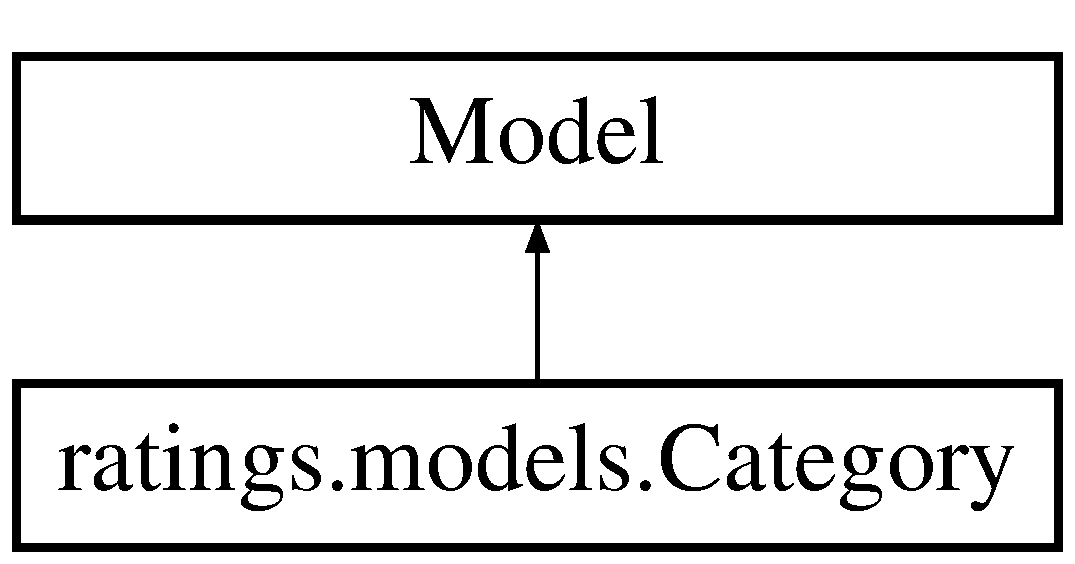
\includegraphics[height=2.000000cm]{classratings_1_1models_1_1Category}
\end{center}
\end{figure}
\subsection*{Public Member Functions}
\begin{DoxyCompactItemize}
\item 
\hypertarget{classratings_1_1models_1_1Category_abeb20d48c9ce44ca777c3adc34f6e50c}{def {\bfseries \-\_\-\-\_\-str\-\_\-\-\_\-}}\label{classratings_1_1models_1_1Category_abeb20d48c9ce44ca777c3adc34f6e50c}

\end{DoxyCompactItemize}
\subsection*{Static Public Attributes}
\begin{DoxyCompactItemize}
\item 
\hypertarget{classratings_1_1models_1_1Category_a82fc31efdb861f55e12c05bacd4436b1}{tuple {\bfseries name} = models.\-Char\-Field(max\-\_\-length=30, unique=True)}\label{classratings_1_1models_1_1Category_a82fc31efdb861f55e12c05bacd4436b1}

\item 
\hypertarget{classratings_1_1models_1_1Category_a22aa60b3b6e97175d01b7ea33af7b2d1}{tuple {\bfseries desc} = models.\-Text\-Field()}\label{classratings_1_1models_1_1Category_a22aa60b3b6e97175d01b7ea33af7b2d1}

\end{DoxyCompactItemize}


\subsection{Detailed Description}
\begin{DoxyVerb}Category class
\end{DoxyVerb}
 

The documentation for this class was generated from the following file\-:\begin{DoxyCompactItemize}
\item 
models.\-py\end{DoxyCompactItemize}

\hypertarget{classratings_1_1forms_1_1CategoryNominationForm}{\section{ratings.\-forms.\-Category\-Nomination\-Form Class Reference}
\label{classratings_1_1forms_1_1CategoryNominationForm}\index{ratings.\-forms.\-Category\-Nomination\-Form@{ratings.\-forms.\-Category\-Nomination\-Form}}
}
Inheritance diagram for ratings.\-forms.\-Category\-Nomination\-Form\-:\begin{figure}[H]
\begin{center}
\leavevmode
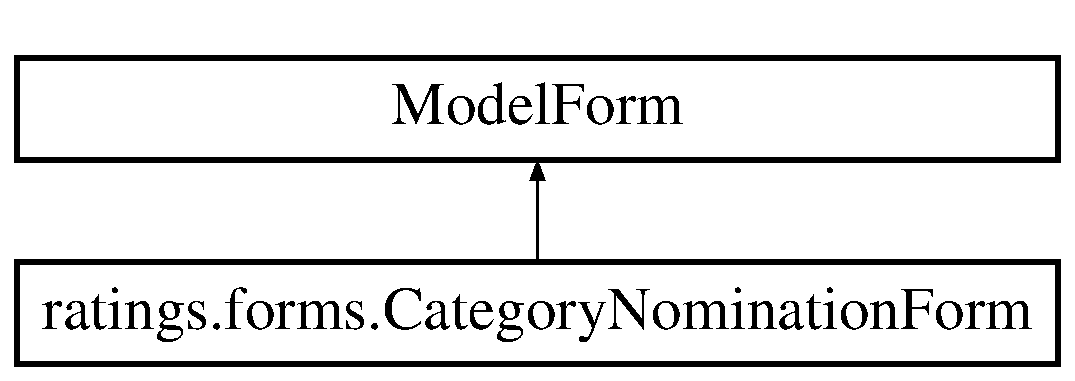
\includegraphics[height=2.000000cm]{classratings_1_1forms_1_1CategoryNominationForm}
\end{center}
\end{figure}
\subsection*{Classes}
\begin{DoxyCompactItemize}
\item 
class \hyperlink{classratings_1_1forms_1_1CategoryNominationForm_1_1Meta}{Meta}
\end{DoxyCompactItemize}
\subsection*{Static Public Attributes}
\begin{DoxyCompactItemize}
\item 
\hypertarget{classratings_1_1forms_1_1CategoryNominationForm_a9bfacd7cd84ce93a9ffa0767edc62ec1}{tuple {\bfseries nominator\-\_\-name} = forms.\-Char\-Field(max\-\_\-length=30)}\label{classratings_1_1forms_1_1CategoryNominationForm_a9bfacd7cd84ce93a9ffa0767edc62ec1}

\item 
\hypertarget{classratings_1_1forms_1_1CategoryNominationForm_a48673d290cfba7c288c7e0eeac0e4f3d}{tuple {\bfseries nominator\-\_\-email} = forms.\-Email\-Field(max\-\_\-length=30)}\label{classratings_1_1forms_1_1CategoryNominationForm_a48673d290cfba7c288c7e0eeac0e4f3d}

\end{DoxyCompactItemize}


\subsection{Detailed Description}
\begin{DoxyVerb}CategoryNominationForm ModelForm (based on Category Model)
\end{DoxyVerb}
 

The documentation for this class was generated from the following file\-:\begin{DoxyCompactItemize}
\item 
forms.\-py\end{DoxyCompactItemize}

\hypertarget{classratings_1_1forms_1_1HorizRadioRenderer}{\section{ratings.\-forms.\-Horiz\-Radio\-Renderer Class Reference}
\label{classratings_1_1forms_1_1HorizRadioRenderer}\index{ratings.\-forms.\-Horiz\-Radio\-Renderer@{ratings.\-forms.\-Horiz\-Radio\-Renderer}}
}
Inheritance diagram for ratings.\-forms.\-Horiz\-Radio\-Renderer\-:\begin{figure}[H]
\begin{center}
\leavevmode
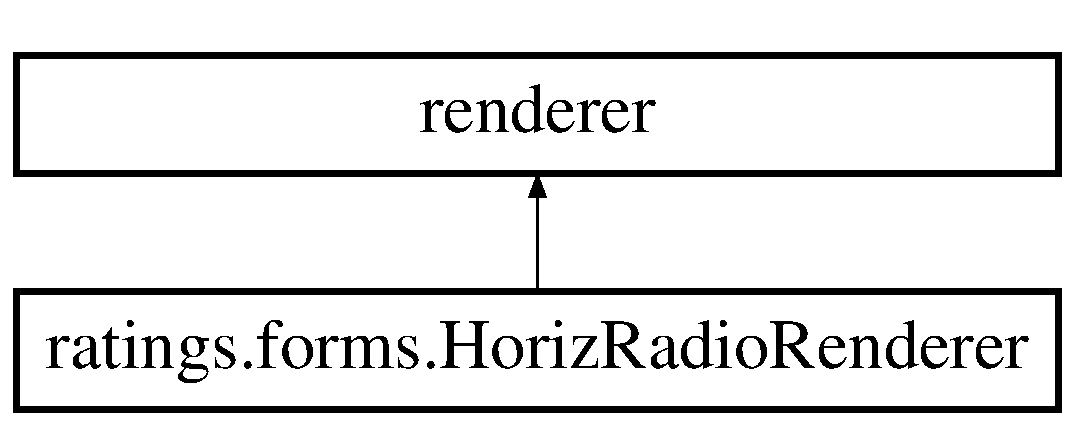
\includegraphics[height=2.000000cm]{classratings_1_1forms_1_1HorizRadioRenderer}
\end{center}
\end{figure}
\subsection*{Public Member Functions}
\begin{DoxyCompactItemize}
\item 
\hypertarget{classratings_1_1forms_1_1HorizRadioRenderer_a90b7fcd9d823c2c87b337a27c23b9326}{def {\bfseries render}}\label{classratings_1_1forms_1_1HorizRadioRenderer_a90b7fcd9d823c2c87b337a27c23b9326}

\end{DoxyCompactItemize}


\subsection{Detailed Description}
\begin{DoxyVerb}class to display radio buttons
\end{DoxyVerb}
 

The documentation for this class was generated from the following file\-:\begin{DoxyCompactItemize}
\item 
forms.\-py\end{DoxyCompactItemize}

\hypertarget{classratings_1_1forms_1_1CategoryNominationForm_1_1Meta}{\section{ratings.\-forms.\-Category\-Nomination\-Form.\-Meta Class Reference}
\label{classratings_1_1forms_1_1CategoryNominationForm_1_1Meta}\index{ratings.\-forms.\-Category\-Nomination\-Form.\-Meta@{ratings.\-forms.\-Category\-Nomination\-Form.\-Meta}}
}
\subsection*{Static Public Attributes}
\begin{DoxyCompactItemize}
\item 
\hypertarget{classratings_1_1forms_1_1CategoryNominationForm_1_1Meta_ab88933a7fa8bc152829c9ab99a4e3207}{{\bfseries model} = Category}\label{classratings_1_1forms_1_1CategoryNominationForm_1_1Meta_ab88933a7fa8bc152829c9ab99a4e3207}

\item 
\hypertarget{classratings_1_1forms_1_1CategoryNominationForm_1_1Meta_ac157756ae5bc45b0faa0c9a7da02e33d}{tuple {\bfseries fields} = ('name', 'desc', 'nominator\-\_\-name', 'nominator\-\_\-email')}\label{classratings_1_1forms_1_1CategoryNominationForm_1_1Meta_ac157756ae5bc45b0faa0c9a7da02e33d}

\item 
\hypertarget{classratings_1_1forms_1_1CategoryNominationForm_1_1Meta_a108a54d1ed5a5e3073fdf8892b3707b2}{dictionary {\bfseries widgets} = \{'desc'\-: forms.\-Textarea(attrs=\{'cols'\-: 35, 'rows'\-: 3\})\}}\label{classratings_1_1forms_1_1CategoryNominationForm_1_1Meta_a108a54d1ed5a5e3073fdf8892b3707b2}

\item 
dictionary {\bfseries labels}
\end{DoxyCompactItemize}


\subsection{Member Data Documentation}
\hypertarget{classratings_1_1forms_1_1CategoryNominationForm_1_1Meta_afe382d7e6bbec1613ca42e1a0897ae48}{\index{ratings\-::forms\-::\-Category\-Nomination\-Form\-::\-Meta@{ratings\-::forms\-::\-Category\-Nomination\-Form\-::\-Meta}!labels@{labels}}
\index{labels@{labels}!ratings::forms::CategoryNominationForm::Meta@{ratings\-::forms\-::\-Category\-Nomination\-Form\-::\-Meta}}
\subsubsection[{labels}]{\setlength{\rightskip}{0pt plus 5cm}dictionary ratings.\-forms.\-Category\-Nomination\-Form.\-Meta.\-labels\hspace{0.3cm}{\ttfamily [static]}}}\label{classratings_1_1forms_1_1CategoryNominationForm_1_1Meta_afe382d7e6bbec1613ca42e1a0897ae48}
{\bfseries Initial value\-:}
\begin{DoxyCode}
1 = \{\textcolor{stringliteral}{'name'}: \textcolor{stringliteral}{"Category Name"}, \textcolor{stringliteral}{'desc'}: \textcolor{stringliteral}{"Category Description"}, \(\backslash\)
2             \textcolor{stringliteral}{'nominator\_name'}: \textcolor{stringliteral}{"Your Name"}, \textcolor{stringliteral}{'nominator\_email'}: \textcolor{stringliteral}{"Your email"}, \(\backslash\)
3             \textcolor{stringliteral}{'free'}: \textcolor{stringliteral}{"Is the tool free to use?&nbsp"}, \(\backslash\)
4             \textcolor{stringliteral}{'online'}: \textcolor{stringliteral}{"Is the tool web-based?&nbsp"}\}
\end{DoxyCode}


The documentation for this class was generated from the following file\-:\begin{DoxyCompactItemize}
\item 
forms.\-py\end{DoxyCompactItemize}

\hypertarget{classratings_1_1forms_1_1VoteForm_1_1Meta}{\section{ratings.\-forms.\-Vote\-Form.\-Meta Class Reference}
\label{classratings_1_1forms_1_1VoteForm_1_1Meta}\index{ratings.\-forms.\-Vote\-Form.\-Meta@{ratings.\-forms.\-Vote\-Form.\-Meta}}
}
\subsection*{Static Public Attributes}
\begin{DoxyCompactItemize}
\item 
\hypertarget{classratings_1_1forms_1_1VoteForm_1_1Meta_a35547c426ff6efd87351a80d1d6af337}{{\bfseries model} = Vote}\label{classratings_1_1forms_1_1VoteForm_1_1Meta_a35547c426ff6efd87351a80d1d6af337}

\item 
\hypertarget{classratings_1_1forms_1_1VoteForm_1_1Meta_a53c7794e98b0e8030e7533836796bffa}{list {\bfseries C\-H\-O\-I\-C\-E\-S} = \mbox{[}(1, 1), (2, 2), (3, 3), (4, 4), (5, 5)\mbox{]}}\label{classratings_1_1forms_1_1VoteForm_1_1Meta_a53c7794e98b0e8030e7533836796bffa}

\item 
tuple {\bfseries fields}
\item 
dictionary {\bfseries widgets}
\item 
dictionary {\bfseries labels}
\end{DoxyCompactItemize}


\subsection{Member Data Documentation}
\hypertarget{classratings_1_1forms_1_1VoteForm_1_1Meta_a181e07f4455cd11384602b077cd16070}{\index{ratings\-::forms\-::\-Vote\-Form\-::\-Meta@{ratings\-::forms\-::\-Vote\-Form\-::\-Meta}!fields@{fields}}
\index{fields@{fields}!ratings::forms::VoteForm::Meta@{ratings\-::forms\-::\-Vote\-Form\-::\-Meta}}
\subsubsection[{fields}]{\setlength{\rightskip}{0pt plus 5cm}tuple ratings.\-forms.\-Vote\-Form.\-Meta.\-fields\hspace{0.3cm}{\ttfamily [static]}}}\label{classratings_1_1forms_1_1VoteForm_1_1Meta_a181e07f4455cd11384602b077cd16070}
{\bfseries Initial value\-:}
\begin{DoxyCode}
1 = (\textcolor{stringliteral}{'overall\_rating'}, \textcolor{stringliteral}{'qual\_of\_doc'}, \(\backslash\)
2             \textcolor{stringliteral}{'efficacy'}, \textcolor{stringliteral}{'usability'}, \textcolor{stringliteral}{'comment'})
\end{DoxyCode}
\hypertarget{classratings_1_1forms_1_1VoteForm_1_1Meta_a80c82dfd8c58f8a74d813043b67b4030}{\index{ratings\-::forms\-::\-Vote\-Form\-::\-Meta@{ratings\-::forms\-::\-Vote\-Form\-::\-Meta}!labels@{labels}}
\index{labels@{labels}!ratings::forms::VoteForm::Meta@{ratings\-::forms\-::\-Vote\-Form\-::\-Meta}}
\subsubsection[{labels}]{\setlength{\rightskip}{0pt plus 5cm}dictionary ratings.\-forms.\-Vote\-Form.\-Meta.\-labels\hspace{0.3cm}{\ttfamily [static]}}}\label{classratings_1_1forms_1_1VoteForm_1_1Meta_a80c82dfd8c58f8a74d813043b67b4030}
{\bfseries Initial value\-:}
\begin{DoxyCode}
1 = \{
2             \textcolor{stringliteral}{'overall\_rating'}: \textcolor{stringliteral}{"Overall Rating"}, \(\backslash\)
3             \textcolor{stringliteral}{'qual\_of\_doc'}: \textcolor{stringliteral}{"Quality of Documentation"}, \textcolor{stringliteral}{'efficacy'}: \textcolor{stringliteral}{"Efficacy"}, \(\backslash\)
4             \textcolor{stringliteral}{'usability'}: \textcolor{stringliteral}{"Usability"}, \textcolor{stringliteral}{'comment'}: \textcolor{stringliteral}{"Optional Comments:&nbsp"}\}
\end{DoxyCode}
\hypertarget{classratings_1_1forms_1_1VoteForm_1_1Meta_a06f1bcb74e8d8c3661382ca14eddfcf1}{\index{ratings\-::forms\-::\-Vote\-Form\-::\-Meta@{ratings\-::forms\-::\-Vote\-Form\-::\-Meta}!widgets@{widgets}}
\index{widgets@{widgets}!ratings::forms::VoteForm::Meta@{ratings\-::forms\-::\-Vote\-Form\-::\-Meta}}
\subsubsection[{widgets}]{\setlength{\rightskip}{0pt plus 5cm}dictionary ratings.\-forms.\-Vote\-Form.\-Meta.\-widgets\hspace{0.3cm}{\ttfamily [static]}}}\label{classratings_1_1forms_1_1VoteForm_1_1Meta_a06f1bcb74e8d8c3661382ca14eddfcf1}
{\bfseries Initial value\-:}
\begin{DoxyCode}
1 = \{
2             \textcolor{stringliteral}{'overall\_rating'}: forms.RadioSelect(\(\backslash\)
3                 renderer = HorizRadioRenderer, choices = CHOICES), 
4             \textcolor{stringliteral}{'qual\_of\_doc'}: forms.RadioSelect(\(\backslash\)
5                 renderer = HorizRadioRenderer, choices = CHOICES), 
6             \textcolor{stringliteral}{'efficacy'}: forms.RadioSelect(\(\backslash\)
7                 renderer = HorizRadioRenderer, choices = CHOICES), 
8             \textcolor{stringliteral}{'usability'}: forms.RadioSelect(\(\backslash\)
9                 renderer = HorizRadioRenderer, choices = CHOICES),
10             \textcolor{stringliteral}{'comment'}: forms.Textarea(attrs=\{\textcolor{stringliteral}{'cols'}: 35, \textcolor{stringliteral}{'rows'}: 3\})\}
\end{DoxyCode}


The documentation for this class was generated from the following file\-:\begin{DoxyCompactItemize}
\item 
forms.\-py\end{DoxyCompactItemize}

\hypertarget{classratings_1_1forms_1_1ToolNominationForm_1_1Meta}{\section{ratings.\-forms.\-Tool\-Nomination\-Form.\-Meta Class Reference}
\label{classratings_1_1forms_1_1ToolNominationForm_1_1Meta}\index{ratings.\-forms.\-Tool\-Nomination\-Form.\-Meta@{ratings.\-forms.\-Tool\-Nomination\-Form.\-Meta}}
}
\subsection*{Static Public Attributes}
\begin{DoxyCompactItemize}
\item 
\hypertarget{classratings_1_1forms_1_1ToolNominationForm_1_1Meta_a572b63db259c55f4106cee3e4cf6226e}{{\bfseries model} = Tool}\label{classratings_1_1forms_1_1ToolNominationForm_1_1Meta_a572b63db259c55f4106cee3e4cf6226e}

\item 
\hypertarget{classratings_1_1forms_1_1ToolNominationForm_1_1Meta_aca5439f4f5c821d07bf5481b4cedab96}{tuple {\bfseries link} = forms.\-Char\-Field(max\-\_\-length=100)}\label{classratings_1_1forms_1_1ToolNominationForm_1_1Meta_aca5439f4f5c821d07bf5481b4cedab96}

\item 
tuple {\bfseries fields}
\item 
\hypertarget{classratings_1_1forms_1_1ToolNominationForm_1_1Meta_a691d68ae9f3eaf5573aa3d0968756de3}{dictionary {\bfseries widgets} = \{'desc'\-: forms.\-Textarea(attrs=\{'cols'\-: 35, 'rows'\-: 3\})\}}\label{classratings_1_1forms_1_1ToolNominationForm_1_1Meta_a691d68ae9f3eaf5573aa3d0968756de3}

\end{DoxyCompactItemize}


\subsection{Member Data Documentation}
\hypertarget{classratings_1_1forms_1_1ToolNominationForm_1_1Meta_a1193d82ba3689ee8fcd68dc919d9b375}{\index{ratings\-::forms\-::\-Tool\-Nomination\-Form\-::\-Meta@{ratings\-::forms\-::\-Tool\-Nomination\-Form\-::\-Meta}!fields@{fields}}
\index{fields@{fields}!ratings::forms::ToolNominationForm::Meta@{ratings\-::forms\-::\-Tool\-Nomination\-Form\-::\-Meta}}
\subsubsection[{fields}]{\setlength{\rightskip}{0pt plus 5cm}tuple ratings.\-forms.\-Tool\-Nomination\-Form.\-Meta.\-fields\hspace{0.3cm}{\ttfamily [static]}}}\label{classratings_1_1forms_1_1ToolNominationForm_1_1Meta_a1193d82ba3689ee8fcd68dc919d9b375}
{\bfseries Initial value\-:}
\begin{DoxyCode}
1 = (\textcolor{stringliteral}{'name'}, \textcolor{stringliteral}{'desc'}, \textcolor{stringliteral}{'link'}, \textcolor{stringliteral}{'free'}, \textcolor{stringliteral}{'online'}, \textcolor{stringliteral}{'category'}, \(\backslash\)
2             \textcolor{stringliteral}{'nominator\_name'}, \textcolor{stringliteral}{'nominator\_email'})
\end{DoxyCode}


The documentation for this class was generated from the following file\-:\begin{DoxyCompactItemize}
\item 
forms.\-py\end{DoxyCompactItemize}

\hypertarget{classratings_1_1models_1_1Tool}{\section{ratings.\-models.\-Tool Class Reference}
\label{classratings_1_1models_1_1Tool}\index{ratings.\-models.\-Tool@{ratings.\-models.\-Tool}}
}
Inheritance diagram for ratings.\-models.\-Tool\-:\begin{figure}[H]
\begin{center}
\leavevmode
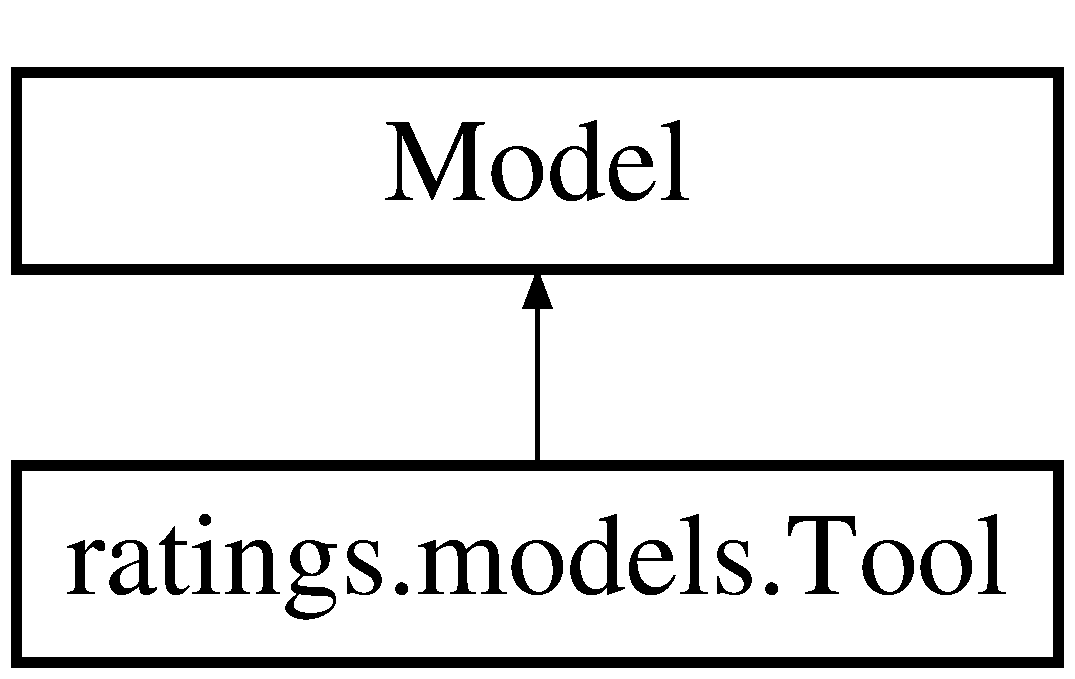
\includegraphics[height=2.000000cm]{classratings_1_1models_1_1Tool}
\end{center}
\end{figure}
\subsection*{Public Member Functions}
\begin{DoxyCompactItemize}
\item 
\hypertarget{classratings_1_1models_1_1Tool_a28bd2c668cea9a1f3eef17dbab22e619}{def {\bfseries \-\_\-\-\_\-str\-\_\-\-\_\-}}\label{classratings_1_1models_1_1Tool_a28bd2c668cea9a1f3eef17dbab22e619}

\end{DoxyCompactItemize}
\subsection*{Static Public Attributes}
\begin{DoxyCompactItemize}
\item 
\hypertarget{classratings_1_1models_1_1Tool_ad7e6ebee671f9b4145dd123d76e5c962}{tuple {\bfseries name} = models.\-Char\-Field(max\-\_\-length=30, unique = True)}\label{classratings_1_1models_1_1Tool_ad7e6ebee671f9b4145dd123d76e5c962}

\item 
\hypertarget{classratings_1_1models_1_1Tool_a5ec493b5bd4afd861a83a66db0847030}{tuple {\bfseries desc} = models.\-Text\-Field()}\label{classratings_1_1models_1_1Tool_a5ec493b5bd4afd861a83a66db0847030}

\item 
\hypertarget{classratings_1_1models_1_1Tool_a299f46aea6d493df3bb5f6eff3026883}{tuple {\bfseries link} = models.\-U\-R\-L\-Field(max\-\_\-length=100)}\label{classratings_1_1models_1_1Tool_a299f46aea6d493df3bb5f6eff3026883}

\item 
\hypertarget{classratings_1_1models_1_1Tool_a2c589f3883eacc0fa48d35a829794d16}{tuple {\bfseries overall\-\_\-rating} = models.\-Decimal\-Field(max\-\_\-digits=4, decimal\-\_\-places=3)}\label{classratings_1_1models_1_1Tool_a2c589f3883eacc0fa48d35a829794d16}

\item 
\hypertarget{classratings_1_1models_1_1Tool_ade202b8bd31fefd0044c2967c02fa39e}{tuple {\bfseries qual\-\_\-of\-\_\-doc} = models.\-Decimal\-Field(max\-\_\-digits=4, decimal\-\_\-places=3)}\label{classratings_1_1models_1_1Tool_ade202b8bd31fefd0044c2967c02fa39e}

\item 
\hypertarget{classratings_1_1models_1_1Tool_ac9bd0bd88e124f61ecb4573f5706cdcb}{tuple {\bfseries efficacy} = models.\-Decimal\-Field(max\-\_\-digits=4, decimal\-\_\-places=3)}\label{classratings_1_1models_1_1Tool_ac9bd0bd88e124f61ecb4573f5706cdcb}

\item 
\hypertarget{classratings_1_1models_1_1Tool_a067bdd59eb8dc016c81389ebd88de0d3}{tuple {\bfseries usability} = models.\-Decimal\-Field(max\-\_\-digits=4, decimal\-\_\-places=3)}\label{classratings_1_1models_1_1Tool_a067bdd59eb8dc016c81389ebd88de0d3}

\item 
\hypertarget{classratings_1_1models_1_1Tool_adb37e2c651865f5231b810ef0a6b03da}{tuple {\bfseries free} = models.\-Boolean\-Field(default=False)}\label{classratings_1_1models_1_1Tool_adb37e2c651865f5231b810ef0a6b03da}

\item 
\hypertarget{classratings_1_1models_1_1Tool_afd85b4aad531988e7ec52d2be2a03b0c}{tuple {\bfseries online} = models.\-Boolean\-Field(default=False)}\label{classratings_1_1models_1_1Tool_afd85b4aad531988e7ec52d2be2a03b0c}

\end{DoxyCompactItemize}


\subsection{Detailed Description}
\begin{DoxyVerb}Tool class
\end{DoxyVerb}
 

The documentation for this class was generated from the following file\-:\begin{DoxyCompactItemize}
\item 
models.\-py\end{DoxyCompactItemize}

\hypertarget{classratings_1_1models_1_1ToolCat}{\section{ratings.\-models.\-Tool\-Cat Class Reference}
\label{classratings_1_1models_1_1ToolCat}\index{ratings.\-models.\-Tool\-Cat@{ratings.\-models.\-Tool\-Cat}}
}
Inheritance diagram for ratings.\-models.\-Tool\-Cat\-:\begin{figure}[H]
\begin{center}
\leavevmode
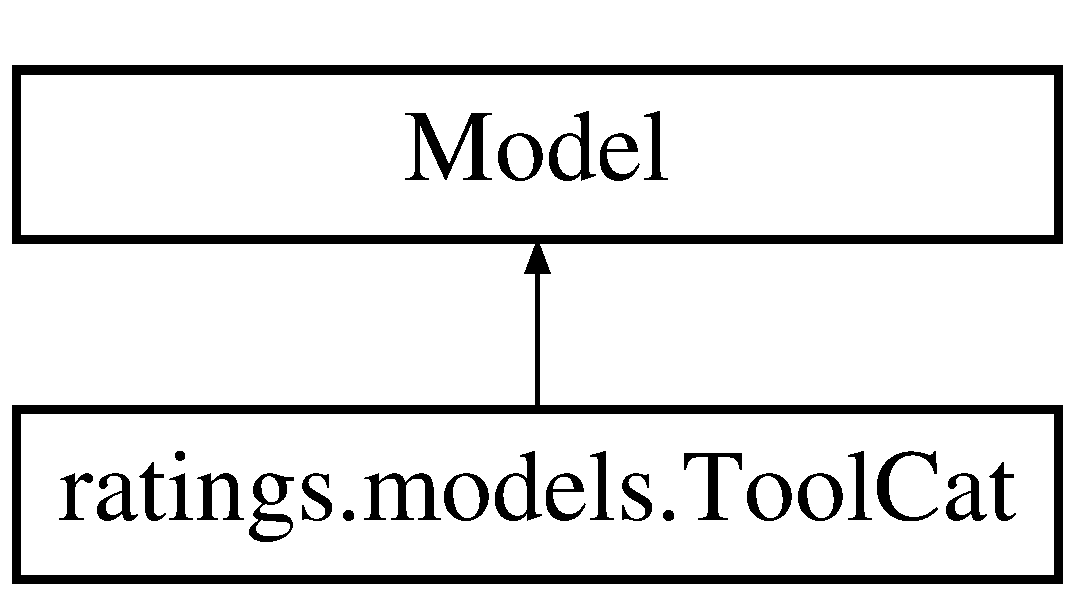
\includegraphics[height=2.000000cm]{classratings_1_1models_1_1ToolCat}
\end{center}
\end{figure}
\subsection*{Public Member Functions}
\begin{DoxyCompactItemize}
\item 
\hypertarget{classratings_1_1models_1_1ToolCat_a3d744035e57606834981035843b9b20e}{def {\bfseries \-\_\-\-\_\-str\-\_\-\-\_\-}}\label{classratings_1_1models_1_1ToolCat_a3d744035e57606834981035843b9b20e}

\end{DoxyCompactItemize}
\subsection*{Static Public Attributes}
\begin{DoxyCompactItemize}
\item 
\hypertarget{classratings_1_1models_1_1ToolCat_ac04b966b5d4a292235c11cff3760ac93}{tuple {\bfseries tool\-\_\-id} = models.\-Foreign\-Key(\hyperlink{classratings_1_1models_1_1Tool}{Tool})}\label{classratings_1_1models_1_1ToolCat_ac04b966b5d4a292235c11cff3760ac93}

\item 
\hypertarget{classratings_1_1models_1_1ToolCat_a6c1906b30c047a2b6fe2a37292dd3242}{tuple {\bfseries cat\-\_\-id} = models.\-Foreign\-Key(\hyperlink{classratings_1_1models_1_1Category}{Category})}\label{classratings_1_1models_1_1ToolCat_a6c1906b30c047a2b6fe2a37292dd3242}

\end{DoxyCompactItemize}


\subsection{Detailed Description}
\begin{DoxyVerb}Tool class
\end{DoxyVerb}
 

The documentation for this class was generated from the following file\-:\begin{DoxyCompactItemize}
\item 
models.\-py\end{DoxyCompactItemize}

\hypertarget{classratings_1_1forms_1_1ToolNominationForm}{\section{ratings.\-forms.\-Tool\-Nomination\-Form Class Reference}
\label{classratings_1_1forms_1_1ToolNominationForm}\index{ratings.\-forms.\-Tool\-Nomination\-Form@{ratings.\-forms.\-Tool\-Nomination\-Form}}
}
Inheritance diagram for ratings.\-forms.\-Tool\-Nomination\-Form\-:\begin{figure}[H]
\begin{center}
\leavevmode
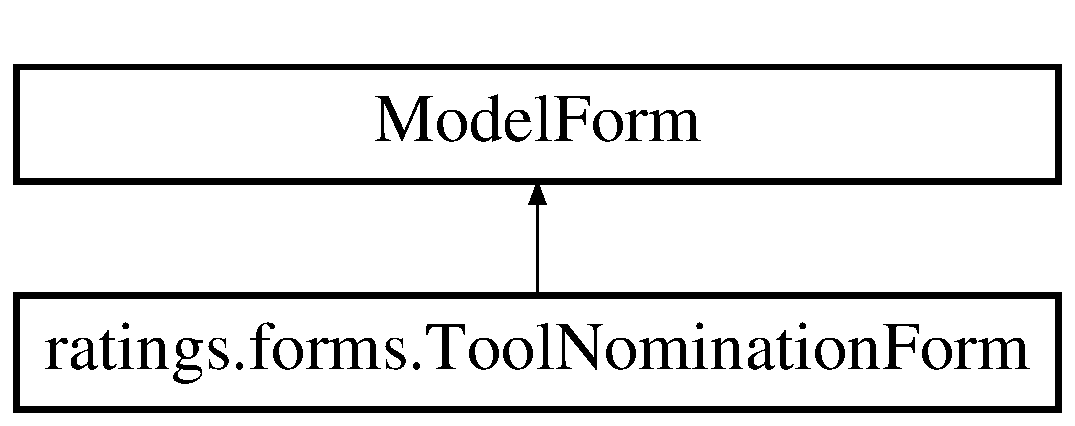
\includegraphics[height=2.000000cm]{classratings_1_1forms_1_1ToolNominationForm}
\end{center}
\end{figure}
\subsection*{Classes}
\begin{DoxyCompactItemize}
\item 
class \hyperlink{classratings_1_1forms_1_1ToolNominationForm_1_1Meta}{Meta}
\end{DoxyCompactItemize}
\subsection*{Static Public Attributes}
\begin{DoxyCompactItemize}
\item 
\hypertarget{classratings_1_1forms_1_1ToolNominationForm_aa7d72b9ca22d5bb212b8a4fd6675e8c5}{tuple {\bfseries category} = forms.\-Char\-Field(max\-\_\-length=100)}\label{classratings_1_1forms_1_1ToolNominationForm_aa7d72b9ca22d5bb212b8a4fd6675e8c5}

\item 
\hypertarget{classratings_1_1forms_1_1ToolNominationForm_a47bba4737e0facbf3fb26009d1169964}{tuple {\bfseries nominator\-\_\-name} = forms.\-Char\-Field(max\-\_\-length=30)}\label{classratings_1_1forms_1_1ToolNominationForm_a47bba4737e0facbf3fb26009d1169964}

\item 
\hypertarget{classratings_1_1forms_1_1ToolNominationForm_a274a9b153d8ac39909d8f8a837ba4994}{tuple {\bfseries nominator\-\_\-email} = forms.\-Email\-Field(max\-\_\-length=30)}\label{classratings_1_1forms_1_1ToolNominationForm_a274a9b153d8ac39909d8f8a837ba4994}

\end{DoxyCompactItemize}


\subsection{Detailed Description}
\begin{DoxyVerb}ToolNominationForm ModelForm (based on Tool Model)
\end{DoxyVerb}
 

The documentation for this class was generated from the following file\-:\begin{DoxyCompactItemize}
\item 
forms.\-py\end{DoxyCompactItemize}

\hypertarget{classratings_1_1models_1_1Vote}{\section{ratings.\-models.\-Vote Class Reference}
\label{classratings_1_1models_1_1Vote}\index{ratings.\-models.\-Vote@{ratings.\-models.\-Vote}}
}
Inheritance diagram for ratings.\-models.\-Vote\-:\begin{figure}[H]
\begin{center}
\leavevmode
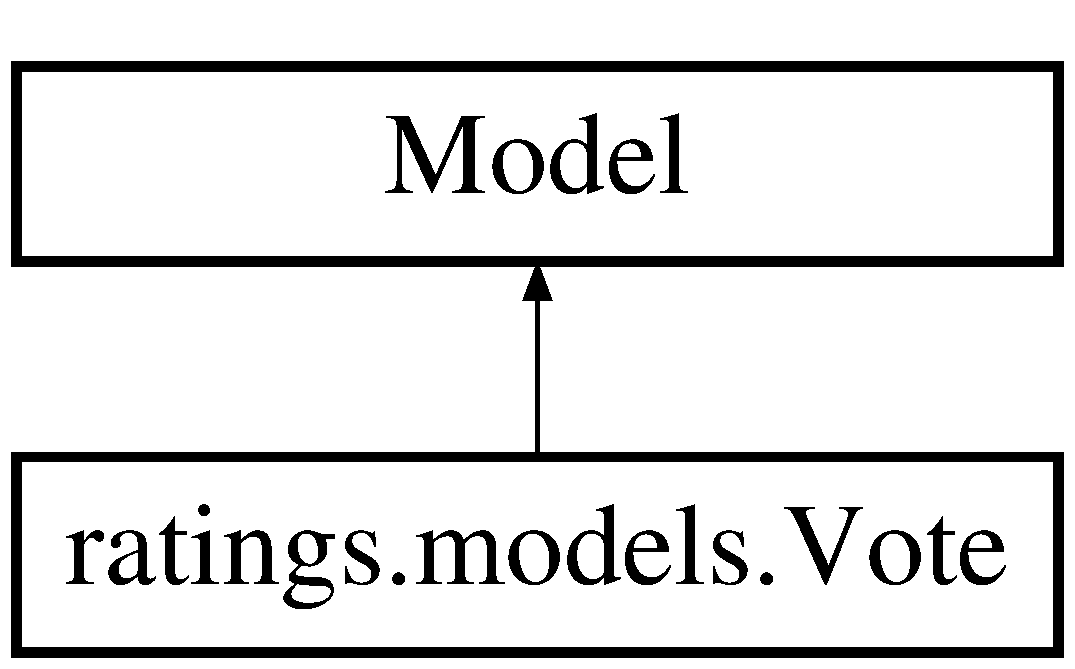
\includegraphics[height=2.000000cm]{classratings_1_1models_1_1Vote}
\end{center}
\end{figure}
\subsection*{Public Member Functions}
\begin{DoxyCompactItemize}
\item 
\hypertarget{classratings_1_1models_1_1Vote_a04c02c7dbcb684592cead310fb9c52fc}{def {\bfseries \-\_\-\-\_\-str\-\_\-\-\_\-}}\label{classratings_1_1models_1_1Vote_a04c02c7dbcb684592cead310fb9c52fc}

\end{DoxyCompactItemize}
\subsection*{Static Public Attributes}
\begin{DoxyCompactItemize}
\item 
\hypertarget{classratings_1_1models_1_1Vote_a6d90101efcb95c4ad9b482dbe0ab4f45}{tuple {\bfseries tool\-\_\-id} = models.\-Foreign\-Key(\hyperlink{classratings_1_1models_1_1Tool}{Tool})}\label{classratings_1_1models_1_1Vote_a6d90101efcb95c4ad9b482dbe0ab4f45}

\item 
\hypertarget{classratings_1_1models_1_1Vote_a144209022f3867968a8bc063c61de5dc}{tuple {\bfseries comment} = models.\-Text\-Field(blank = True)}\label{classratings_1_1models_1_1Vote_a144209022f3867968a8bc063c61de5dc}

\item 
\hypertarget{classratings_1_1models_1_1Vote_abab964e4961f5cabc5b562057cd24608}{tuple {\bfseries review\-\_\-date} = models.\-Date\-Time\-Field()}\label{classratings_1_1models_1_1Vote_abab964e4961f5cabc5b562057cd24608}

\item 
\hypertarget{classratings_1_1models_1_1Vote_a668e499a155103447842694cc3c5519b}{tuple {\bfseries overall\-\_\-rating} = models.\-Positive\-Small\-Integer\-Field()}\label{classratings_1_1models_1_1Vote_a668e499a155103447842694cc3c5519b}

\item 
\hypertarget{classratings_1_1models_1_1Vote_aa6d51b455e4177bb442766ccea14b54c}{tuple {\bfseries qual\-\_\-of\-\_\-doc} = models.\-Positive\-Small\-Integer\-Field()}\label{classratings_1_1models_1_1Vote_aa6d51b455e4177bb442766ccea14b54c}

\item 
\hypertarget{classratings_1_1models_1_1Vote_afea6bd04715f329357f0ab948db263bc}{tuple {\bfseries efficacy} = models.\-Positive\-Small\-Integer\-Field()}\label{classratings_1_1models_1_1Vote_afea6bd04715f329357f0ab948db263bc}

\item 
\hypertarget{classratings_1_1models_1_1Vote_a41d3762f8deb83dcb8938fa1115ce740}{tuple {\bfseries usability} = models.\-Positive\-Small\-Integer\-Field()}\label{classratings_1_1models_1_1Vote_a41d3762f8deb83dcb8938fa1115ce740}

\end{DoxyCompactItemize}


\subsection{Detailed Description}
\begin{DoxyVerb}Vote model
\end{DoxyVerb}
 

The documentation for this class was generated from the following file\-:\begin{DoxyCompactItemize}
\item 
models.\-py\end{DoxyCompactItemize}

\hypertarget{classratings_1_1forms_1_1VoteForm}{\section{ratings.\-forms.\-Vote\-Form Class Reference}
\label{classratings_1_1forms_1_1VoteForm}\index{ratings.\-forms.\-Vote\-Form@{ratings.\-forms.\-Vote\-Form}}
}
Inheritance diagram for ratings.\-forms.\-Vote\-Form\-:\begin{figure}[H]
\begin{center}
\leavevmode
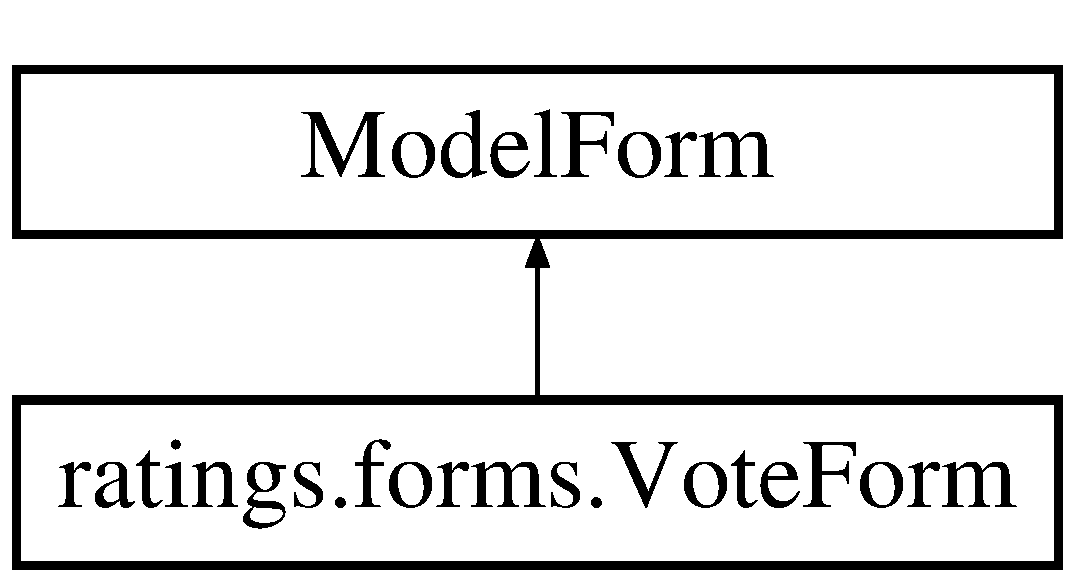
\includegraphics[height=2.000000cm]{classratings_1_1forms_1_1VoteForm}
\end{center}
\end{figure}
\subsection*{Classes}
\begin{DoxyCompactItemize}
\item 
class \hyperlink{classratings_1_1forms_1_1VoteForm_1_1Meta}{Meta}
\end{DoxyCompactItemize}


\subsection{Detailed Description}
\begin{DoxyVerb}# VoteForm ModelForm (based on Vote Model)
\end{DoxyVerb}
 

The documentation for this class was generated from the following file\-:\begin{DoxyCompactItemize}
\item 
forms.\-py\end{DoxyCompactItemize}

%--- End generated contents ---

% Index
\newpage
\phantomsection
\addcontentsline{toc}{chapter}{Index}
\printindex

\end{document}
